\documentclass{article}
\usepackage{amsmath}
\usepackage[utf8]{inputenc}
\usepackage{graphicx}
\usepackage{verbatim}
\usepackage{float}
\usepackage[makeroom]{cancel}
\usepackage[english]{babel}
\usepackage{textcomp}
\usepackage{gensymb}
\usepackage{color}
\usepackage{subcaption}
\usepackage{caption}
\usepackage{hyperref}
\usepackage{physics}
\usepackage{dsfont}
%\usepackage{amsfonts}
\usepackage{listings}
\usepackage{multicol}
\usepackage{units}

% From Eirik's .tex
\usepackage{epstopdf}
\usepackage{cite}
\usepackage{braket}
\usepackage{url}
\bibliographystyle{plain}

\usepackage{algorithmicx}
\usepackage{algorithm}% http://ctan.org/pkg/algorithms
\usepackage{algpseudocode}% http://ctan.org/pkg/algorithmicx

\usepackage[margin=1cm]{caption}
\usepackage[outer=1.2in,inner=1.2in]{geometry}
% For writing full-size pages
%\usepackage{geometry}
%\geometry{
%  left=5mm,
%  right=5mm,
%  top=5mm,
%  bottom=5mm,
%  heightrounded,
%}

% Finding overfull \hbox
\overfullrule=2cm

\lstset{language=IDL}
 %\lstset{alsolanguage=c++}
\lstset{basicstyle=\ttfamily\small}
 %\lstset{backgroundcolor=\color{white}}
\lstset{frame=single}
\lstset{stringstyle=\ttfamily}
\lstset{keywordstyle=\color{red}\bfseries}
\lstset{commentstyle=\itshape\color{blue}}
\lstset{showspaces=false}
\lstset{showstringspaces=false}
\lstset{showtabs=false}
\lstset{breaklines}
\lstset{aboveskip=20pt,belowskip=20pt}

\lstset{basicstyle=\footnotesize, basewidth=0.5em}
\lstdefinestyle{cl}{frame=none,basicstyle=\ttfamily\small}
\lstdefinestyle{pr}{frame=single,basicstyle=\ttfamily\small}
\lstdefinestyle{prt}{frame=none,basicstyle=\ttfamily\small}
% \lstinputlisting[language=Python]{filename}


\definecolor{codepurple}{rgb}{0.58,0,0.82}
\definecolor{backcolour}{rgb}{0.95,0.95,0.92}
\definecolor{dkgreen}{rgb}{0,0.6,0}
\definecolor{gray}{rgb}{0.5,0.5,0.5}
\definecolor{magenta}{rgb}{0.58,0,0.82}

\lstdefinestyle{pystyle}{
  language=Python,
  aboveskip=3mm,
  belowskip=3mm,
  columns=flexible,
  basicstyle={\small\ttfamily},
  backgroundcolor=\color{backcolour},
  commentstyle=\color{dkgreen},
  keywordstyle=\color{magenta},
  numberstyle=\tiny\color{gray},
  stringstyle=\color{codepurple},
  basicstyle=\footnotesize,
  breakatwhitespace=false,
  breaklines=true,
  captionpos=b,
  keepspaces=true,
  numbers=left,
  numbersep=5pt,
  showspaces=false,
  showstringspaces=false,
  showtabs=false,
  tabsize=2
}

%%%%%%%%%%%%%%%%%%%%%%%%%%%%%%%%
% Self made macros here yaaaaaay
\newcommand\answer[1]{\underline{\underline{#1}}}
\newcommand\pd[2]{\frac{\partial #1}{\partial #2}}
\newcommand\red[1]{\textcolor{red}{\textbf{#1}}}
\newcommand\numberthis{\addtocounter{equation}{1}\tag{\theequation}}
% Usage: \numberthis \label{name}
% Referencing: \eqref{name}

% Some matrices
\newcommand\smat[1]{\big(\begin{smallmatrix}#1\end{smallmatrix}\big)}
\newcommand\ppmat[1]{\begin{pmatrix}#1\end{pmatrix}}

%%%%%%%%%%%%%%%%%%%%%%%%%%%%%%%%%
% Eirik's self made macros
\newcommand{\s}{^{*}}
\newcommand{\V}[1]{\mathbf{#1}}
\newcommand{\husk}[1]{\color{red} #1 \color{black}}
\newcommand{\E}[1]{\cdot 10^{#1}}
\newcommand{\e}[1]{\ \text{#1}}
\newcommand{\tom}[1]{\big( #1 \big)}
\newcommand{\Tom}[1]{\Big( #1 \Big)}
\newcommand{\tomH}[1]{\big[ #1 \big] }
\newcommand{\TomH}[1]{\Big[ #1 \Big]}
\newcommand{\tomK}[1]{ \{ #1 \} }
\newcommand{\TomK}[1]{\Big\lbrace #1 \Big\rbrace}
\newcommand{\bigabs}[1]{\left| #1 \right|}

% Section labeling
\usepackage{titlesec}% http://ctan.org/pkg/titlesec
\renewcommand{\thesubsection}{\arabic{subsection}}


% Title/name/date
\title{FYS4150 - Project 2}
\author{Simen Nyhus Bastnes \& Eirik Ramsli Hauge}
\date{3. October 2016}

\begin{document}
\maketitle
\begin{abstract}
The aim of this project is to solve Schrödinger's equation for two electrons with and without a repulsive Coulomb interaction in a three-dimensional harmonic oscillator well. We start by reformulating the equation in a discretized form as an eigenvalue equation, which can be solved with Jacobi's method. The program will include unit tests and time measurement comparing Jacobi's method to another method. We found that Jacobi's method became more accurate if we started out with a bigger matrix, but it also became very slow with increasing n. The probability of finding the electrons over a bigger $\rho$ interval decreases as $\omega_r$ increases, but if we add the Coulomb interaction the interval will be larger than for its non-Coulomb counterpart.
\end{abstract}
\subsection{Introduction}
We started by first studying one then two electrons in a harmonic oscillator well and by solving the Schrödinger's equation by reformulating it in a discretized form as an eigenvalue equation and solving that equation with Jacobi's method. \\
Once the Schrödinger's equation was on a form we can solve with Jacobi's method, we will solve it for $n$x$n$ matrices of different size for one electron and compare our results. Then we will see if the number of rotations needed to complete Jacobi's method can be apporximated by a polynomal and compare the time usage of our "home made" Jacobi's method with the time usage of Armadillos solver for eigenvalues. \\ \\
Afterwards we will increase the number of electrons to two. We change our harmonic oscillator potential to make it dependent on $\omega_r$, reflecting the strength of the potential. The Coulomb interaction will also be implemented in this part of the program, so that we can compare the probability $|\Psi(\rho)|^2$ for different $\omega_r$ with and without Coulomb interaction. \\ \\
The program will also include three unit tests checking if we get the right eigenvalues, find the largest non-diagonal element and if orthogonality is preserved during Jacobi's method. 


%In project 2, we aim to solve Schrödinger's equation for two electrons with and %without a repulsive Coulomb interaction in a three-dimensional harmonic oscillator %well. We start by reformulating the equation in a discretized form as an eigenvalue %equation, which can be solved with Jacobi's method. \\\\We can then compare our %implementation Jacobi's method fares against ``smarter'' algorithms for solving %eigenvalue equations. Finally, we will look at implementing unit-tests, in order to %test that the various parts of our program does what it's intended to do.\\\\
%\red{Should maybe be rewritten, or changed order, or add more, dunno}

%%%%%%%%%%%%%%%%%%%%%%%%%%%%%%%%%%%%%%%%%%%%%%%%%%%%%%%%%%%%%%
\subsection{Theory}
\subsubsection{Schrödinger's equation}
In this project, we will assume that the electrons move in a three-dimensional harmonic oscillator potential, and repel each other via the static Coulomb interaction. By assuming spherical symmetry, the solution for the radial part of Schrödinger's equation for one electron reads
\begin{align*}
  -\frac{\hbar^2}{2m}\bigg(\frac{1}{r^2}\frac{d}{dr}r^2\frac{d}{dr} - \frac{l(l+1)}{r^2}\bigg)R(r) + V(r)R(r) = ER(r)\numberthis\label{eq:radial_schroedinger}
\end{align*}
For the rest of the project, we set the orbital momentum quantum number $l$ to zero. In our non-interacting case, the harmonic oscillator potential is $V(r) = (1/2)kr^2$ with $k=m\omega^2$.\\\\We perform a substitution for $R(r) = (1/r)u(r)$, introduce a dimensionless variable $\rho = (1/\alpha)r$, where $\alpha$ is a constant with dimension length $\alpha = (\hbar^2/mk)^{1/4}$. Inserting this into the Scrödinger equation \eqref{eq:radial_schroedinger}, we get
\begin{align*}
-\frac{d^2}{d\rho^2}u(\rho) + \rho^2u(\rho) = \lambda u(\rho)\numberthis\label{eq:dimless_schroedinger}
\end{align*}
where $\lambda = (2m\alpha^2/\hbar^2)E$. Equation \eqref{eq:dimless_schroedinger} is the first equation we want to solve numerically, and we will later use that for $l=0$, the first eigenvalues $\lambda$ are $\lambda_0 = 3$, $\lambda_1 = 7$ and $\lambda_2 = 11$.\\\\
Starting our journey to write equation \eqref{eq:dimless_schroedinger} as an eigenvalue equation, we use the by now standard expression for the second derivative
\begin{align*}
  u'' = \frac{u(\rho+h)-2u(\rho)+u(\rho-h)}{h^2}+\mathcal{O}(h^2)
\end{align*}
where $h$ is our step length. We define minimum and maximum values for $\rho$, $\rho_{\text{min}} = 0$ and $\rho_{\text{max}}$, as we cannot set $\rho_{\text{max}} = \infty$. When setting $\rho_{\text{max}}$, we need to make sure that it is set high enough so that the square of the wavefunction $u$ is small near $\rho_{\text{max}}$ for accuracy of the solution. Next, we split this interval into $N$ number of mesh points, so that we can define the step length as
\begin{align*}
  h = \frac{\rho_N-\rho_0}{N}
\end{align*}
where $\rho_0 = \rho_{\text{min}}$ and $\rho_{\text{max}} =\rho_N$. This gives us an expression for $\rho$ at point $i$
\begin{align*}
  \rho_i = \rho_0 + ih\;\;\;\;\;\;\;\;\;i=1,2,\dots,N
\end{align*}
Now we can rewrite the second derivative as
\begin{align*}
  u_i'' = \frac{u_{i+1}-2u_i + u_{i-1}}{h^2}
\end{align*}
Using this, we can rewrite the dimensionless Schrödinger equation \eqref{eq:dimless_schroedinger} as a discretized equation.
\begin{align*}
  -\frac{u_{i+1}-2u_i+u_{i-1}}{h^2} + \rho_i^2u_i = -\frac{u_{i+1}-2u_i+u_{i-1}}{h^2} + V_iu_i = \lambda u_i \numberthis\label{eq:discretized_schroedinger}
\end{align*}
where $V_i = \rho_i^2$ is the harmonic oscillator potential. From the previous project, we recall that we can represent equation \eqref{eq:discretized_schroedinger} in terms of a tridiagonal matrix, where the diagonal elements are given by
\begin{align*}
  d_i = \frac{2}{h^2} + V_i = \frac{2}{h^2} + \rho_i^2
\end{align*}
and the non-diagonal matrix elements
\begin{align*}
  e_i = -\frac{1}{h^2}
\end{align*}
We notice that in this case, the non-diagonal matrix elements are constant. Using this, we can now write the Schrödinger equation as
\begin{align*}
  d_iu_i + e_{i-1}u_{i-1} + e_{i+1}u_{i+1} = \lambda u_i
\end{align*}
So that we now have the following eigenvalue equation
\begin{align*}
\ppmat{\frac{2}{h^2}+V_1&-\frac{1}{h^2}&0&\dots&0\\
    -\frac{1}{h^2}&\frac{2}{h^2}+V_2&-\frac{1}{h^2}&0&\dots\\
    \dots&\dots&\dots&\dots&0\\
    \dots&\dots&-\frac{1}{h^2}&\frac{2}{h^2}+V_{N-2}&-\frac{1}{h^2}\\
    0&\dots&0&-\frac{1}{h^2}&\frac{2}{h^2}+V_{N-1}}
  \ppmat{u_1\\u_2\\\dots\\u_{N-2}\\u_{N-1}} = \lambda
  \ppmat{u_1\\u_2\\\dots\\u_{N-2}\\u_{N-1}} \numberthis\label{eq:eigval_eq}
\end{align*}
which is what we want to solve by using Jacobi's method.

%%%%%%%%%%%%%%%%%%%%%%%%%%%%%%%%%%%%%%%%%%%%%%%%%%%%%%%%%%
\subsubsection*{Interacting case}
The eigenvalue equation \eqref{eq:eigval_eq} was derived by assuming one electron in a harmonic oscillator potential. For two electrons with no repulsive Coulomb interaction, we have the following Schrödinger equation
\begin{align*}
  \bigg(-\frac{\hbar^2}{2m}\frac{d^2}{dr_1^2} - \frac{\hbar^2}{2m}\frac{d^2}{dr_2^2} + \frac{1}{2}kr_1^2 + \frac{1}{2}kr_2^2\bigg)u(r_1,r_2) = E^{(2)}u(r_1,r_2)
\end{align*}
With no interaction, this can be written out as the product of two single-electron wave functions, like we did earlier. Introducing relative coordinates $\mathbf{r} = \mathbf{r_1} - \mathbf{r_2}$ and center-of-mass coordinate $\mathbf{R} = 1/2(\mathbf{r_1}+\mathbf{r_2})$, and adding the repulsive Coulomb interaction between the two electrons to our potential
\begin{align*}
  V(r_1,r_2) = \frac{\beta e^2}{|\mathbf{r_1}-\mathbf{r_2}|} = \frac{\beta e^2}{r}
\end{align*}
So that we get the following radial Schrödinger equation (omitting the center-of-mass motion)
\begin{align*}
  \bigg(-\frac{\hbar^2}{m}\frac{d^2}{dr^2} + \frac{1}{4}kr^2 + \frac{\beta e^2}{r}\bigg)\psi(r) = E_r\psi(r)\\
\end{align*}
This is quite similar to the equation \eqref{eq:radial_schroedinger} we found earlier, and we can likewise introduce a dimensionless variable $\rho = r/\alpha$, and rewrite Schrödinger's equation as
\begin{align*}
  -\frac{d^2}{d\rho^2}\psi(\rho) + \omega_r^2\rho^2\psi(\rho) + \frac{1}{\rho}\psi(\rho) = \lambda\psi(\rho)
\end{align*}
So we see that the only thing we have to modify when adding the repulsive coloumb interaction is to change the potential from $\rho^2$ to $\omega_r\rho^2 + 1/\rho$, where we treat $\omega_r$ as a parameter reflecting the strength of the harmonic oscillator potential. We will later look at how the wave function behaves for different values of $\omega_r$.
%%%%%%%%%%%%%%%%%%%%%%%%%%%%%%%%%%%%%%%%%%%%%%%%%%%%%%%%%%%%

\subsubsection{Jacobi's method}
The aim of Jacobi's method is to use similarity transformation to make a $n \times n$ matrix into a diagonal $n \times n$ matrix with its eigenvalues as the diagonal. We do this by starting with a matrix $\V{A}$ which is diagonally dominant \cite{DDMatrix}. Within this matrix we find the largest element that is not on the diagonal, calling its indexes $k$ and $l$. The algorithm goes as follows:
\begin{algorithm}[H]
\small
\caption{Maximum non-diagonal element}\label{alg:max_offdiag}
\begin{algorithmic}[1]
\State $max = 0.0$
\For{$i=0,\,n$}
\For{$j= i+1, \, n$}
\If{$|A[i][j]| > max$}
\State{$|A[i][j]| = max$}
\State{k = i}
\State{l = j}
\EndIf
\EndFor
\EndFor
\end{algorithmic}
\end{algorithm}
Now we want to rotate matrix $\V{A}$ such that the larges off-diagonal element becomes zero. This is done by using equation:
\begin{equation}
\V{B} = \V{S}^{\V{T}} \V{A} \V{S}
\label{eq:symtrans}
\end{equation}
Where $\V{S}$ is given as:
\begin{align*}
\ppmat{1 & 0 & \cdots & 0 & 0 & \cdots & 0 & 0 \\
	   0 & 1 & \cdots & 0 & 0 & \cdots & 0 & 0 \\
	   \vdots & \vdots & \ddots & \vdots & \vdots & \vdots & \vdots & \vdots \\
	   0 & 0 & \cdots & \cos \theta & 0 & \cdots & 0 & \sin \theta \\
	   0 & 0 & \cdots & 0 & 1 & \cdots & 0 & 0 \\
	   \vdots & \vdots & \vdots & \vdots & \vdots & \ddots & \vdots & \vdots \\
	   0 & 0 & \cdots & 0 & 0 & \cdots & 1 & 0 \\
	   0 & 0 & \cdots & -\sin \theta & 0 & \cdots & 0 & \cos \theta \\}
\end{align*}
With properties $\V{S}^{\V{T}} = \V{S}^{-1}$.
The positioning of $\cos \theta$ and $\sin \theta$ within the matrix is defined by the index of the largest off-digaonal element like this:
\begin{align*}
s_{kk} = s_{ll} = \cos\theta , \quad s_{kl} = -s_{lk} = \sin \theta, \quad s_{ii} = -s_{_ii} = 1 \quad i \neq k, \, i \neq l
\end{align*}
This is the same as performing a plane rotation on A around an angle $\theta$ in the Euclidean $n$-dimensional space. \\
For $\V{B}$ this gives us:
\begin{align*}
				b_{ii} 	&= a_{ii}, \ i \neq k, \ i \neq l \\
				b_{ik} 	&= a_{ik}\cos \theta - a_{il}\sin\theta,\ i \neq k, \ i \neq l \\
				b_{il} 	&= a_{il} \cos\theta + a_{ik}\sin\theta, \ i \neq k, \ i \neq l \\
				b_{kk} 	&= a_{kk}\cos^2\theta - 2a_{kl}\cos\theta \sin\theta + a_{ll}\sin^2\theta \\
				b_{ll} 	&= a_{ll}\cos^2\theta +2a_{kl}\cos\theta\sin\theta + a_{kk}\sin^2\theta \\
				b_{kl} 	&= (a_{kk} - a_{ll})\cos\theta \sin\theta +a_{kl}(\cos^2\theta - \sin^2\theta)
\end{align*}
Where $\theta$ is set as the angle that makes $b_{kl} = 0$. Each transformation can be proven to bring the matrix closer to the diagonal form. \cite{lecturenotes}  \\ \\
When all this is done, the old maxmium off-diagonal value will have become zero and a new one will have risen, but it will not be as large as the old one. We repeat our whole process until the maxmium value of all off-diagonal elements are below a certain threshold value. Ideally we would want them all to be zero, but very, very small values is good enough. \\
By looking at our expression for $b_kl = 0$ and defining
\begin{align*}
t = \tan\theta &= \frac{\sin\theta}{\cos\theta} \\
\tau = \cot 2\theta &= \frac{a_{ll} - a_{kk}}{2a_{kl}}
\end{align*}
We get:
\begin{align*}
(a_{kk} - a_{ll})\cos\theta \sin\theta +a_{kl}(\cos^2\theta - \sin^2\theta) &= 0 \\
(a_{kk} - a_{ll})\cos^2\theta t + a_{kl}\cos^2\theta - a_{kl}\sin^2\theta &= 0 \\
(a_{kk} - a_{ll}) t + a_{kl} - a_{kl}\frac{\sin^2\theta}{\cos^2\theta} &= 0 \\
(a_{kk} - a_{ll}) t + a_{kl}(1-t^2) &= 0 \\
\frac{a_{kk} - a_{ll}}{a_{kl}} t &= t^2 -1 \\
-\tau t &= \frac{t^2-1}{2} \\
t^2 + 2 \tau t - 1 = 0, \quad &\Rightarrow \quad t = -\tau \pm \sqrt{1 + \tau^2}
\intertext{Cosine and sinus are easily found to be}
\cos \theta = \frac{1}{\sqrt{1 + t^2}}, \quad& \sin\theta = \cos\theta \cdot t
\end{align*} 
As we can see we can choose two different values for $t$. The one we want is the one that is the smallest. This is evident if we look at $b_{ik}$ and $b_{il}$. Hopefully these values will quickly reach values near zero and  we want to keep them there. To do this we want $\cos \theta$ to go to 1 and $\sin \theta$ to go to 0 simultaniously. By always choosing the lowest $t$-value we choose the lowest possible angle and therefore we will minimize the changes to the non-diagonal elements in the matrix. Except for $b_{kl}$ which is always set to zero. \\ \\

To fully grasp the idea of this method we have imagined it as this: \\
Let us pretend that you have ten bars in front of you to affect one big bar placed in the middle of the ten. These ten bars can be pushed down, but as you push down one, the others will be affected also. We want to push all the bars (except the big one in the middle) as far down as possible, and if you push down the tallest bar, the others can't reach its height, but they are free to go up and down. Then all you have to do is push down one bar (find the maximum non-diagonal element and rotate the matrix) see how the other bars react (view the matrix after rotation), locate the bar that is now the highest and push that one down. As you do this, gradually all the bars will come under a certain height, even though they may not be completely pushed down. When you are satisfied with the shortness of the tallest bar, your job is done and we have found our diagonal matrix with eigenvalues.
%\husk{Jacobi's algorithm here?}

\subsubsection{Unit tests}
We implemented three unit tests. The first checks if Jacobi's method returns the right eigenvalues for a known matrix with known eigenvalues. The second test checks if our function for finding the largest non-diagonal element does so for a known symmetric matrix And the last one checks if the eigenvectors of our rotated matrix are still orthogonal. For the last check we use the fact that for a vector $\V{v}$ that has orthogonal properties:
\begin{align*}
\V{v}_j^{T} \V{v}_i &= \delta_{ij}
\intertext{The vector $\V{w_i} = \V{U}\V{v}_i$ will also be orthogonal after a unitary or orthogonal transformation. This can be showed by the following:}
\V{w}_j^{T} \V{w}_i = \V{v}_j^T \V{U}^T \V{U} \V{v}_i &= \V{v}_j^{T} \V{v}_i = \delta_{ij}
 \end{align*}
This was used by implementing the third method as a part of each step in Jacobi's method when called upon.

%%%%%%%%%%%%%%%%%%%%%%%%%%%%%%%%%%%%%%%%%%%%%%%%%%%%%%%%%%%%%%%%%%%%%%%%%
\subsection{Experimental}
The programs used in this project can be found in the GitHub repository \cite{Github}, in the \texttt{/src/} folder. When running the program, it takes 3 command line arguments, $N$, $\rho_{\text{max}}$ and \texttt{mode}. The program has four different runmodes, which we will discuss in some more detail.
\subsubsection{One electron, non-interacting case}
Setting \texttt{mode} to \texttt{one} runs the program for one electron and no Coulomb interacted, with specified dimension $N$ and maximum value $\rho_{\text{max}}$, and stores the 5 lowest eigenvalues (calculated both by Jacobi's method and Armadillo's \texttt{eig\_sym()} function) in a file \texttt{eigenvalues\_noint\_n<N>.dat}. The execution time for both methods are appended to the file \texttt{timing.txt}.
\subsubsection{Two electrons, interacting case}
Setting \texttt{mode} to \texttt{two-int} runs the program for 4 different values of $\omega_r =$ (0.01, 0.5, 1.0, 5.0) with the Coulomb interaction added.\\The eigenvector for the ground state is written to the file \texttt{eigenvectors\_two-int\_n<N>.dat}
\subsubsection{Two electrons, non-interacting case}
Setting \texttt{mode} to \texttt{two-noint} runs the program for the same values of $\omega_r$ as the interacting case, with no Coulomb interaction.\\The ground state eigenvector is written to the file \texttt{eigenvectors\_two-noint\_n<N>.dat}.
\subsubsection{Unit tests}
Setting \texttt{mode} to \texttt{unit-tests} runs three unit tests on the different modules in our program, and the result from the tests are written to the file \texttt{unittest.txt}.
\subsection{Results}
The results created by the program are stored in the \texttt{/benchmarks/} folder, while plots generated from these text-files are in \texttt{/figures/}. For Jacobi's method, the number of rotations is printed to terminal.

\subsubsection{One Electron in Harmonic Oscillator}
From the part of our program that looks at the non-interactive case for one electron we found our lowest three eigenvalues. The result is presented in table \ref{tab:eigenvalues} where we see the eigevalues as a function of matrix size $n$.
\begin{table}[H]
\centering
\caption{The three lowest eigenvalues for the non interactive case for different $n$-values. $\rho_{max} = 10.$}
\begin{tabular}{c|c|c|c|c|c|c|c} 
n & 10 & 50 & 100 & 200 & 300 & 400 & 500 \\ \hline
$\lambda_1$ & 2.6867 & 2.9874  & 2.9968  & 2.9992  & 2.9996 & 2.9998  & 2.9998 \\ \hline
$\lambda_2$ & 6.1130 & 6.9369  & 6.9843  & 6.9960  & 6.9982 & 6.9990  & 6.9993\\ \hline
$\lambda_3$ & 11.057 & 10.8452 & 10.9617 & 10.9904 & 10.9957& 10.9976 & 10.9984\\ 
\end{tabular}
\label{tab:eigenvalues}
\end{table}
But $n$ is not the only variant, we can also change $\rho_{max}$. In table \ref{tab:rhoeigenvalues} we see how the eigenvalues change as a function of $\rho_{max}$. Here we have used $n = 101$.
\begin{table}[H]
\centering
\caption{The difference in eigenvalues as a function of $\rho_{max}$ at matrix size $n = 101$.}
\begin{tabular}{c|c|c|c|c}
$\rho_{max}$ & 1 & 5 & 10 & 15 \\ \hline
$\lambda_1$ &  9.963  & 2.999  & 2.997  & 2.993 \\ \hline
$\lambda_2$ &  39.023 & 6.996  & 6.985  & 6.965 \\ \hline
$\lambda_3$ &  87.365 & 10.990 & 10.962 & 10.915 \\ 
\end{tabular}
\label{tab:rhoeigenvalues}
\end{table}
Jaobi's method uses a certain number of iterations to reach the point where all non-diagonal numbers are as good as zero. For our program, number of iterations as a function of n is plotted in \ref{fig:iterations} where we have used the limit $\epsilon = 1.0\cdot 10^{-8}$ as a threshold.
\begin{figure}[H]
\centering
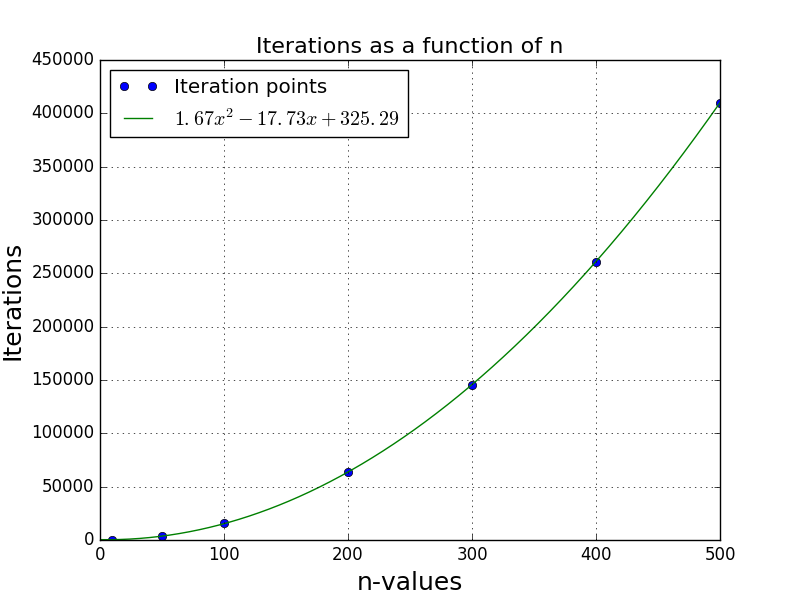
\includegraphics[scale=0.5]{../figures/iterations.png}
\caption{Number of iterations as a function of matrix size $n$.}
\label{fig:iterations}
\end{figure}
In our program we have used two different methods for finding eigenvalues: Jacobi's method and Armadillo. The difference in time for each method is presented in table \ref{tab:time}
\begin{table}[H]
\centering
\caption{The time used by each method with matrix size $n$ and $\rho_{max} = 10$.}
\begin{tabular}{c|c|c}
n & Jacobi [ms] & Armadillo [ms] \\ \hline
10 &  0.27 & 0.65        \\ \hline
50 &  24.48 & 1.34       \\ \hline
100 & 339.93 & 4.79      \\ \hline 
200 & 4609.32 & 34.13    \\ \hline
300 & 27044.07 & 108.31  \\ \hline
400 & 73842.08 & 230.47  \\ \hline
500 & 190636.43 & 436.97 \\ \hline
\end{tabular}
\label{tab:time}
\end{table}

\subsubsection{Two electrons in a harmonic oscillator}
We run our program without the repulsive Coulomb interaction. The eigenvectors for the ground state is shown in figure \ref{fig:eigvec_noint_200}.
\begin{figure}[H]
  \centering
  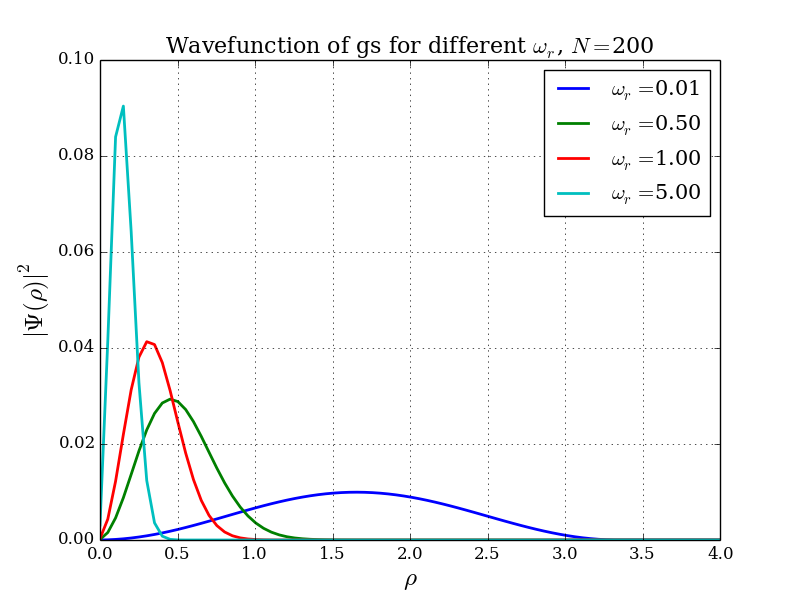
\includegraphics[scale=0.47]{../figures/eigvec_two-noint_n200.png}
  \caption{Plot of the ground state eigenvector for different $\omega_r$ values, without Coulomb interaction, and matrix dimension $N=200$. $\rho_{\text{max}} = 10$, but plotted from $\rho = 0$ to $\rho = 4$ for readability.}
  \label{fig:eigvec_noint_200}
\end{figure}
Running the program with the Coulomb interaction gives us figure \ref{fig:eigvec_int_200}.
\begin{figure}[H]
  \centering
  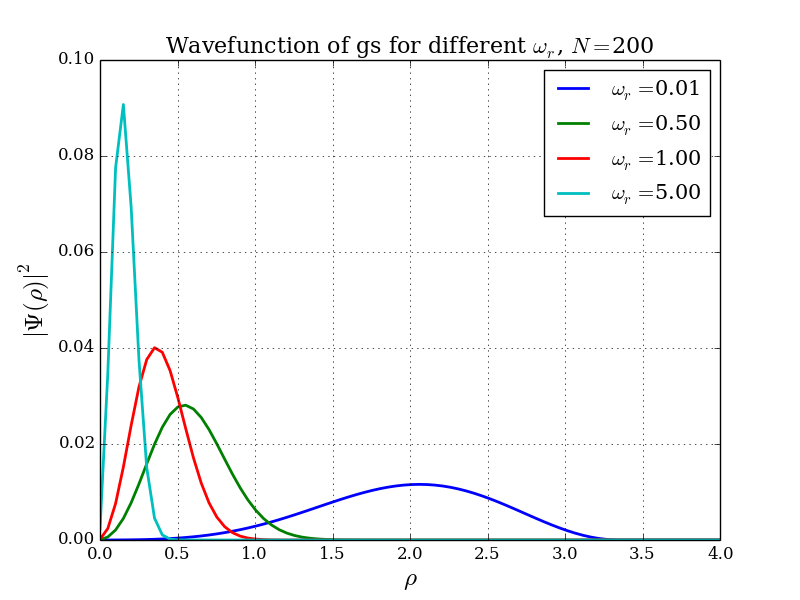
\includegraphics[scale=0.47]{../figures/eigvec_two-int_n200.png}
  \caption{Plot of the ground state eigenvector for different $\omega_r$ values, with repulsive Coulomb interaction, and matrix dimension $N=200$. $\rho_{\text{max}} = 10$, but plotted from $\rho = 0$ to $\rho = 4$ for readability.}
  \label{fig:eigvec_int_200}
\end{figure}
We look a bit closer at figure \ref{fig:eigvec_noint_200} and \ref{fig:eigvec_int_200}, and plot some of the eigenvectors in the same plot.
\begin{figure}[H]
  \centering
  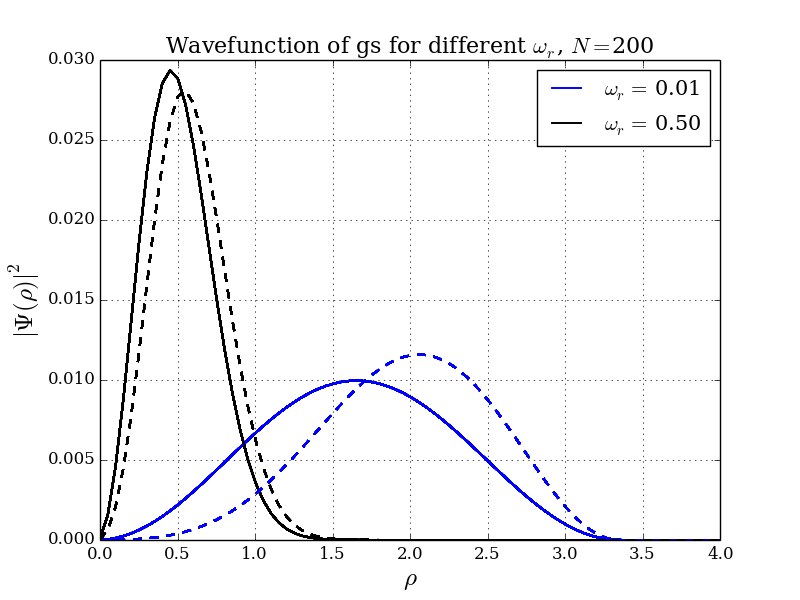
\includegraphics[scale=0.5]{../figures/eigvec_compare_n200.png}
  \caption{Plot of the ground state eigenvectors for $\omega_r = 0.01$ and $\omega_r = 0.5$ and no Coulomb interaction. Overplotted in dashed lines is the corresponding eigenvector with a repulsive Coulomb interaction added.}
  \label{fig:eigvec_compare}
\end{figure}
\subsection{Discussion}
\subsubsection{One Electron in Harmonic Oscillator}
As we can see from table \ref{tab:eigenvalues} the larger matrix we have, the better eigenvalues we get. Our aim was to get four leading digits after the decimal point. But we only achieved this for our lowest eigenvalue. It is clear that for a matrix of size 400x400 the lowest eigenvalue will have four leading digits after the decimal point. The other two are getting nearer four digits, but since we have no repetition of the last digit or the two last digits in respectively the case of $\lambda_2$ and $\lambda_3$ we can not say anything certain. However, the fact that $\lambda_1$ needed $n=400$ and that $\lambda_2$ seems to be very close at $n=500$ should gives us a hint of how big a matrix we would need. If it was very important for us to have all four digits in the case of $\lambda_3$ we would take our time and run the program for higher and higher $n$-values. Since this is not the case, we are satisfied by stopping here.
It is also apparent from table \ref{tab:rhoeigenvalues} that the eigenvalues are also dependent on $\rho_{max}$ which is logical.\\ \\
From figure \ref{fig:iterations} we can see that the number of iterations needed can be approximated as a second degree polynomial as a function of the matrix size $n$. This is logical as the "area" of the matrix will increase as a function of $n^2$ giving the program more to work with. This is not a perfect fit as we have too few iteration points to make a good formula, but it works. Again, if a part of a bigger project was dependent on this part of the program being as accurate as possible, I would run the program for higher values of $n$. \\ \\
Table \ref{tab:time} clearly shows us that our method is timewise inferior compared to the method Armadillo uses. While we have to wait more than 3 minutes for $n = 500$ with Jacobi, it is done in 0.4 seconds with Armadillo. This is because Jacobi is a very brute force way of finding the eigenvectors. While it works, the problem is that when we have found the largest non-diagonal element of the matrix and set it to zero, we are never sure that it won't become the largest again (even though it will never be as large as it was). This means that we have to look over all the non-diagonal elements for every iteration and that we have to work on the same element multiple times. This again leads to a slow method, even though it gives the results we want. Therefore it is important to think of the accuracy of the eigenvalues compared to the time usage. With high $n$ you can get good accuracy, but it will also take more time. Even though we are pretty sure Armadillo always will be correct we can never know. If this program were to be used to find the eigenvalues of many different matrices, we would have to test out many known cases and see if both methods deliver each time.

\subsubsection{Two electrons in a harmonic oscillator}
For our case with two electrons in the harmonic oscillator potential without Coulomb interaction, we look at figure \ref{fig:eigvec_noint_200} to see how the wave function (squared) behaves when varying $\omega_r$. We see that when increasing $\omega_r$, the peak becomes increasingly higher, while the width decreases. From quantum physics, we recall that when plotting $|\psi|^2$, this corresponds to the probability distribution. We can therefore infer from the figure that as $\omega_r$ increases, we are more likely to find the particle closer to $\rho = 0$. This makes a lot of sense, since we earlier said that we treat $\omega_r$ as a parameter reflecting the strength of the harmonic oscillator potential, and increasing it causes the potential well to get stronger.\\\\
Figure \ref{fig:eigvec_int_200} shows the same plot as figure \ref{fig:eigvec_noint_200}, but with a repulsive Coulomb interaction added. It might not be easy to see that much difference between the figures, but if we study them closely, we see that the wave function curves seems to be shifted slightly to the right as compared to without interaction. This would make a lot of sense, as a repulsive interaction between the two electrons should push the electrons apart the closer they are to each other. In doing so, it should counteract (to some degree) the effect of the harmonic oscillator potential.\\\\
To more clearly see this, we can look at figure \ref{fig:eigvec_compare}, where the eigenvectors for the two lowest $\omega_r$ values, with and without interaction is overplotted. Looking at this, we see clearly that when adding the Coulomb interaction, the wave function gets shifted towards the right. We also see that when increasing $\omega_r$, this shift gets smaller, as the harmonic oscillator potential starts to dominate strength wise.
\subsection{Conclusion}
From table \ref{tab:eigenvalues} we can clearly see that the accuracy of the eigenvalues given to us by Jacobi's method is a function of the matrix size $n$. However, from table \ref{tab:time} we can also see that the time used by the program greatly increases with the increasing of $n$. Although we have mostly used Jacobi's method here, Armadillo's eigenvalue finder seems to be the better choice in the future.\\\\
In the two electron case, we see from figure \ref{fig:eigvec_compare} that when adding the repulsive Coulomb interaction, the probability distributions get shifted away from the center, where the harmonic oscillator potential is the strongest, but as strength of potential $\omega_r$ increases, this shift gets smaller.
\bibliography{references}
\end{document}
